\section{Diagramme entité-association}
\begin{figure}[H]
    \centering
    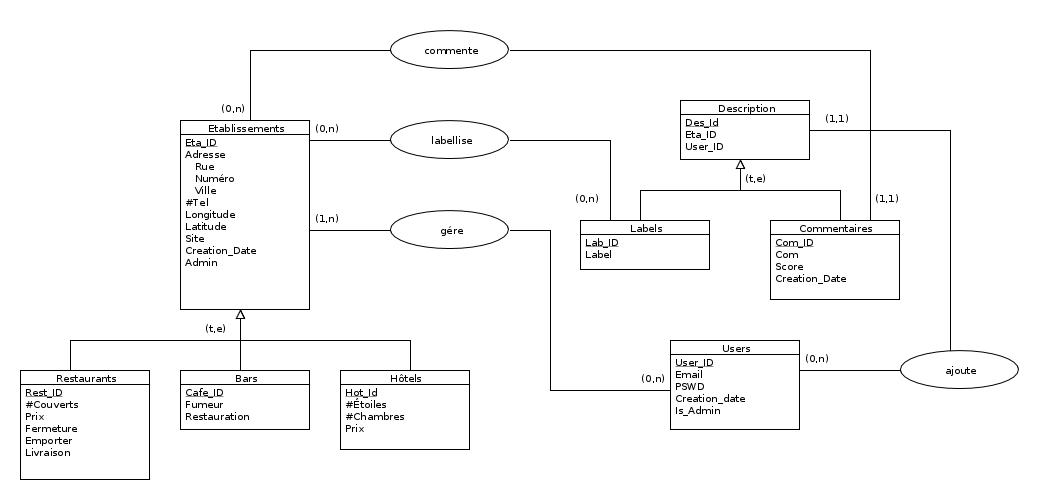
\includegraphics[scale=0.60, angle=90]{diaEA4}
    \caption{Diagramme entité-relation de la base de donnée}
\end{figure}
\subsection{Remarques diagramme}
\begin{itemize}
\item L'entité Descriptions a été ajoutée car des attributs communs sont partagés entre les Commentaires et les Labels (exemple: établissement concerné).
\item Un label peut ne décrire aucun établissement en particulier (dans le cas où le seul établissement qu'il décrit est retiré de la BDD).
\end{itemize}
\subsection{Contraintes d'intégrité}
\begin{itemize}
\item Un utilisateur ne peut pas apposer le même label plusieurs fois sur le même établissement.
\item Le nombre de couvert(s) d'un restaurant doit être strictement supérieur à 0.
\item La date d'enregistrement d'un utilisateur doit être inférieure à la date d'une description ajoutée par cette utilisateur.
\item La date d'enregistrement d'un admin doit être inférieure à la date de création d'un nouvel établissement.
\item Le nombre d'étoiles d'un hôtel doit être compris entre 0 et 5 (inclus).
\item Le score entré par un utilisateur lors d'un commentaire doit être compris entre 0 et 5 (inclus).
\item Le nombre de chambre(s) d'un hôtel doit être strictement supérieur à 0.
\item Un Etablissement.Eta\_ID correspond à exactement soit un Restaurants.Res\_ID, soit un Bars.Bar\_ID, soit un Hotels.Hot\_ID.
\item Un Descriptions.Des\_ID correspond à exactement soit un Labels.Lab\_ID, soit un Commentaires.Com\_ID.
\end{itemize}
\newpage